
\documentclass[11pt]{article}
%\linespread{1.1}
\usepackage{graphicx,import}
\usepackage{amsmath}
\usepackage{setspace}
\usepackage{color}
\usepackage{float}
\usepackage[inkscapelatex=false,inkscapearea=page]{svg}
\onehalfspacing
%\doublespacing

\title {Architecture and Open Queue Model \\ \bigskip \large Thesis}
\author {Silvio Dei Giudici, Marco Morella, Mattia Nicolella}
\date{21 September 2020}

\begin{document}
\maketitle
\section{Introduction}
This section will deal with the assumptions we have made so far and why we've made them. Alternatives will be described for the various possibilities.\\
\subsection{Assumptions}
\begin{enumerate}
\item \textbf{Assumption 1}: All layers have no horizontal connection. The scheme we will present in section 2 will feature LANs accessible by all nodes of the same layer so this type of communication is actually possible through those LANs, but for now decided to not have horizontality in the message system.
\item \textbf{Assumption 2}: The only entity needing a storage system is the Central Node, in particular we are assuming that all other nodes receive information that can be processed, stored and aggregated in the RAM which will never be full. This is a strong assumption that can be relaxed if needed by adding disks in the regional and primary/secondary layer.
\item \textbf{Assumption 3}: The RAM element of the nodes doesn't need its own queue model, indeed it can be modeled in symbiosis with the CPU since it is used by only that component.
\item \textbf{Assumption 4}: In this first stage we won't be holding account of the fault tolerance of the system, in particular we are not considering duplication of the data not in storaging neither in multiple link sending.
\item \textbf{Assumption 5}: Equiprobability of receiving a message on any given level, indeed we will assume that, each time a central sends a message to a node on a level the probability that any one of them is the target is the same, this can be relaxed easily by putting a fixed probability parameter in the formulas.
\item \textbf{Assumption 6}: more of a design choice for the moment, each node is modeled as a simple queue composed of CPU+RAM, in future they will be extended(for example a disk) and may need more component and a review of the entire queue model.
\end{enumerate}
\subsection{Table}
First of all, we started by compiling the table with the responses as we expect them to be. The green ones are those decisions we made while the black ones are trivial ones that have no alternatives.\\
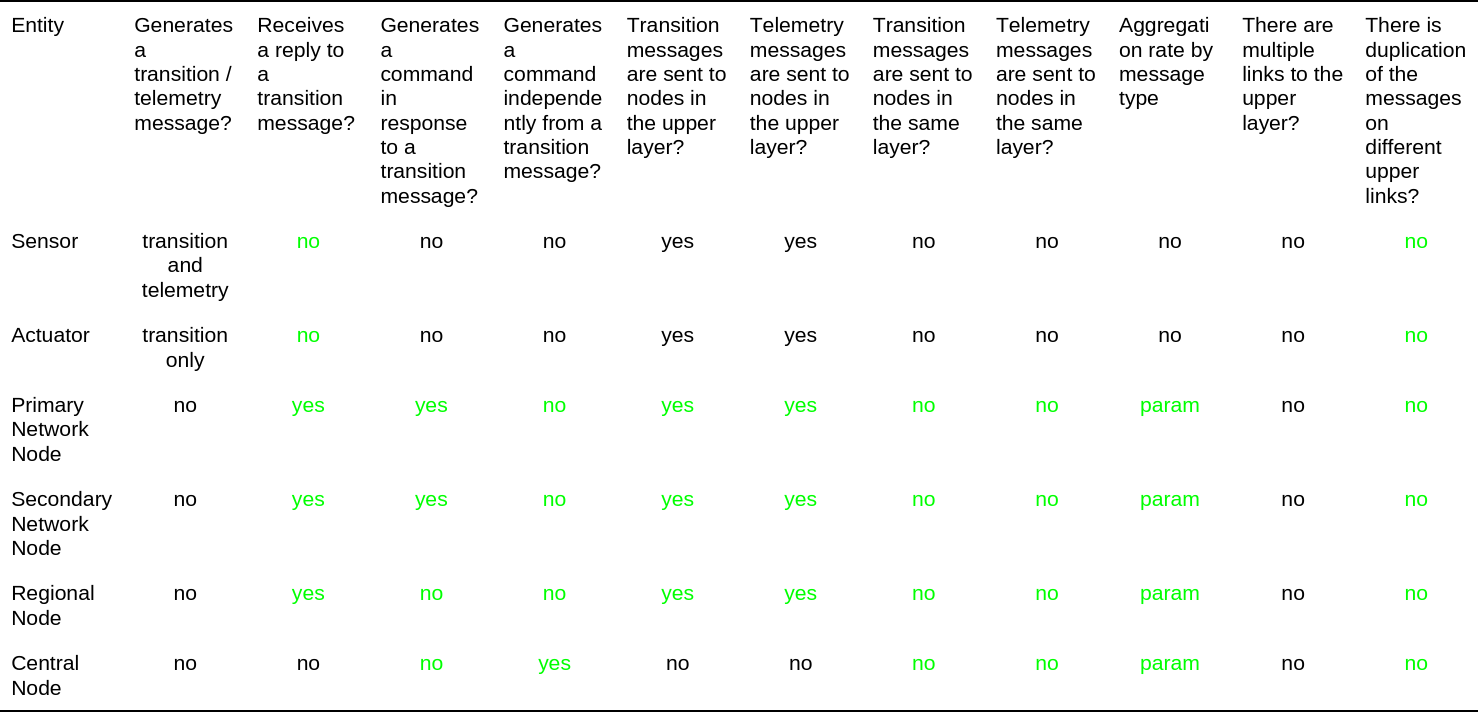
\includegraphics[width=15cm, height=10cm]{table.png}
Now, row by row we will justify or explain our answers:
\begin{enumerate}
\item Generate a transition or telemetry message: the sensor give telemetry informations to the upper node with a certain rate. Both actuators and sensor will generete a transitions message in the case that their state is changed without a transition command received. All others entities have no case in which they need to do so.
\item Receives a reply to a transition message: sensor and actuators don't need an acknowledgment from the upper level, while all other entities do. The only exception is the Central node since he doesn't have an upper node to send to.
\item Generates a command in response to a transition message: the primary reading the transition messages may need to issue commands to actuators in order to keep the system flowing.
\item Generates a command independently from a transition message: none of the entities may generate a command without any trigger, the only exception being the central node which sends commands when needed.
\item Transition messages are sent to nodes in the upper layer: all entities need to send to an upper level until the central node is reached.
\item Telemetry messages are sent to nodes in the upper layer: same as last one.
\item Transition messages are sent to nodes in the same layer: no, for assumption 1.
\item Telemetry messages are sent to nodes in the same layer: no, for assumption 1.
\item Aggregation rate by message type: we don't have the actual rate so we put a parameter in the aggregation formulas.
\item There are multiple links to the upper layer: not useful at the moment for modeling and queue formulas so we skipped over it. Also for Assumption 4 we may implement it in a later stage.
\item There is duplication of the messages on different upper links: No, for assumption 4.
\end{enumerate}

\section{Structural scheme}
This section will explain how the structural scheme for the system is made and its project's choices.\\
In the model we are going to show, we used as connection between the upper level node and the LAN of the lower level nodes a WAN between two routers. An alternative is possible if we transform this WAN into a long distance LAN where only one router is needed for this connection on the upper level node side.\\
The choice of a WAN was made due to the high regional spam that the second level nodes are going to cover.
\begin{figure}[H]
	\hspace*{-3.75cm}
	\centering
  \frame{\includesvg[width=20cm]{centralregional}}
  \caption{Focus on Central and Regional nodes}
\end{figure}
\begin{figure}[H]
	\hspace*{-3.75cm}
	\frame{\includesvg[width=20cm]{primarysecondary}}
	\caption{Focus on Regional and Primary/Secondary nodes}
\end{figure}
Figure 1 represents the connection between Central and Regional nodes, while Figure 2 shows the connection between Regional and Primary/Secondary. We can  see that lower level router is used as an interface for lower level nodes to receive and send messages to the upper level node. Keeping in mind assumption 1 on the horizontal level communication, even if the nodes on a level share a LAN they won't send messages to their peers.\\
\begin{figure}[H]
	\hspace*{-3.75cm}
  \frame{\includesvg[width=20cm]{primarysensor}}
  \caption{Focus on Primary/Secondary nodes and end points}
\end{figure}
Instead in figure 3, which displays the connection between Primary/Secondary nodes and the end points of the edge system, namely actuators and sensors, one LAN is used for each type of connection technology, in this case MANET and WIRELESS, both spanning between end points and their respective upper level node node.\\
Furthermore this iteration is parametric so a central node manages n regional nodes. Each regional node manages m primary and k secondary nodes, these parameters varies with the regional node they are associated to. Same thing extends to primary/secondary with respect to the sensors/actuators, respectively in numbers s and a.\\
One last note about the scheme is that at the moment we divided on two LANs primary and secondary for clarity since they have different rate, operations and technology. Likewise for the different communication technology with actuators and sensors.\\
The whole scheme:
\begin{figure}[H]
	\hspace*{-3.75cm}
	\frame{\includesvg[width=20cm]{structural_scheme_wan}}
  \caption{Structural scheme}
\end{figure}

\section{Queues Scheme and Formulas}
The following open queue scheme will be divided in segments during the analysis of each queue.
\begin{figure}[H]
	\vspace*{-0.5cm}
	\hspace*{-3.5cm}
	\centering
	\frame{\includesvg[width=25cm, height=19cm]{queue_network_wan}}
	\caption{The open queue scheme}
\end{figure}
\subsection{Classes}
Based on the specifics and the architecture, we opted for a multi-class open queueing model, in particular at the moment we have three different classes going through the system:
\begin{itemize}
\item t: telemetry events, where a sensors sends to its superior the data it has periodically, this data then will be aggregated at each level up until the central node.
\item e: transition events, which are sent by actuators and sensors when the network state changes.
\item c: command events, generated either indipendently by the central node when managing the network or by a primary node in response to a transition message from one of its sensors/actuators.
\end{itemize}
Another type of message flowing through the network is a reply message but since they are triggered only by transition events we aggregated them in the visits.
Due to the nature of this kind of open queueing model, the formulas regarding Utilization factor, system demand and response time are given.

\subsection{Notation}
We will deline the notation in the following formulas, each of them has one or many subscripts for the item they refer to, the same type of element in a different part has the same notation even though it's not the same element:
\begin{itemize}
\item $\lambda_t$, $\lambda_e$, $\lambda_c$: $\lambda$ is the arrival rate, respectively for the data type telemetry, transition and command.
\item $V$: mean number of visits.
\item $S$: service time.
\item $D$: service demand.
\item $U$: utilization factor.
\item $R$: response time.
\end{itemize}
The elements we are going to analyze are:
\begin{itemize}
\item cn : central node.
\item cns : central node storage
\item rn : regional node.
\item pn : primary node.
\item sn : secondary node.
\item wl : wireless.
\item mt : manet.
\item pl : primary lan.
\item sl : secondary lan.
\item ps : primary-secondary lan.
\item rl : regional lan.
\item cl : central lan.
\end{itemize}
Each node has a summary section which describes the total response time for that node type.\\
We will navigate the queue network starting from the sensors and actuators and until reaching the central node.

\begin{figure}[H]
	\centering
	\frame{\includesvg[width=20cm, height=17cm]{queue_network_wireless_manet}}
	\caption{Focus on actuators, sensors,  primary/secondary nodes, wireless and MANET LANs}
\end{figure}

\subsection{Actuators and Sensors}
Sensors at the moment don't receive any command, we still have drawn them as queues for future extensions while actuators are defined by the rates.\\

\subsection{WIRELESS/MANET Lan}
The first element we are going to look at is the WIRELESS lan. At this stage we are not considering the implication of the different technology thus we will only show the formulas for Wireless and the Manet's formulas will be mirrored.\\
For the formulas we used the assumption 5 on equiprobability and the table presented in section 1.2, in particular the first four columns.\\
The mean number of visits is trivially one for telemetry and commands since only one messages goes through the LAN, it's two for transition since a reply is needed.\\
More interesting are the formulas regarding the arrival rates.\\
In the telemetry cases the total arrival rate $\lambda_{wl, t}$ is the rate of a single sensor multiplied by the number of sensors.\\
For transition instead, $\lambda_{wl, e}$ will be a sum of two terms, since both actuators and sensors send messages.\\
Finally for $\lambda_{wl, c}$, the first term is the case where the central node issues a command, so the sent command of that class of messages will arrive to an actuator with a certain probability, given the assumption 5 this probability is one over the sum of all possible paths that can be taken by this message: one of the regional node, then one of the primary or secondary node and then one of all the actuators, in this case we are concerned only if they go on the WIRELESS($\frac{a_{wl}}{a_{wl}+a_{mt}}$). The second term instead is the case where a command is prompted due to a transition message so we multiply the arrival rate of transition event for primary or secondary node by a probability of the transition to generate a command, divided by two because the two paths, WIRELESS or MANET, we are assuming that the message has the same probability to flow over the two networks. It is a strong assumption and may need to be relaxed in future work.\\
\begin{equation}
    \begin{array}{l}
        V_{wl, t} = 1 \\
        V_{wl, e} = 2 \\ %reply
        V_{wl,c} = 1 \\
        \lambda_{wl, t} = s*\lambda_{s, t} \\
        \lambda_{wl, e} = s*\lambda_{s, e} + a*\lambda_{a, e} \\
        \lambda_{wl, c} = \frac{1}{n*(m+k)} * \frac{a_{wl}}{a_{wl}+a_{mt}} * \lambda_{cn, c} + prb * \frac{\lambda_{pn, e}}{2}  \\\
    \end{array}
\end{equation}
In the last equation, the second term requires a change from primary node arrival rate to secondary node arrival rate in the case that the upper node is indeed a secondary.\\
From the previous formulas and the open queue model we can compute the Service Demand, Utilization factor and Response time.
\begin{equation}
    \begin{array}{l}
        D_{wl, t} = V_{wl, t} * S_{wl, t} \\
        D_{wl, e} = V_{wl, e} * S_{wl, e} \\
        D_{wl, c} = V_{wl, c} * S_{wl, c} \\
        U_{wl, t} = \lambda_{wl, t} * D_{wl, t} \\
        U_{wl, e} = \lambda_{wl, e} * D_{wl, e} \\
        U_{wl, c} = \lambda_{wl, c} * D_{wl, c} \\
        U_{wl} = U_{wl, t} + U_{wl, e} + U_{wl, c} \\
        R_{wl, t} = \frac{D_{wl, t}}{1 - U_{wl}} \\
        R_{wl, e} = \frac{D_{wl, e}}{1 - U_{wl}} \\
        R_{wl, c} = \frac{D_{wl, c}}{1 - U_{wl}} \\
    \end{array}
\end{equation}

\subsection{Primary Node}
All formulas in this chapter are relatable to the previous one and thus we won't need any note on them.\\
Formulas for secondary nodes are the same as primary ones for now so we will only discuss these one.\\
The equations of the previous element will be used as arrival rates for the primary node thus both MANET and WIRELESS will be referred to.\\
While transitions and telemetries are simply the sum of the rates coming from MANET and WIRELESS, commands need an explanation.\\
Indeed the first term is the rate arriving to a single primary node thus divided by the number of regionals and then by the number of primary plus secondary nodes. The second term is again the probability of dependent commands.
\begin{equation}
    \begin{array}{l}
        V_{pn, t} = 1 \\
        V_{pn, e} = 2 \\ %reply
        V_{pn,c} = 1 \\
        \lambda_{pn, t} = \lambda_{wl, t} + \lambda_{mt, t} \\
        \lambda_{pn, e} = \lambda_{wl, e} + \lambda_{mt, e} \\
        \lambda_{pn, c} = \frac{1}{n} * (\frac{1}{m+k}) * \lambda_{cn, c} + prb * \lambda_{pn, e}  \\\
    \end{array}
\end{equation}
From the previous formulas and the open queue-qui mettiamo anche la WAN model we can compute the Service Demand, Utilization factor and Response time.
\begin{equation}
    \begin{array}{l}
        D_{pn, t} = V_{pn, t} * S_{pn, t} \\
        D_{pn, e} = V_{pn, e} * S_{pn, e} \\
        D_{pn, c} = V_{pn, c} * S_{pn, c} \\
        U_{pn, t} = \lambda_{pn, t} * D_{pn, t} \\
        U_{pn, e} = \lambda_{pn, e} * D_{pn, e} \\
        U_{pn, c} = \lambda_{pn, c} * D_{pn, c} \\
        U_{pn} = U_{pn, t} + U_{pn, e} + U_{pn, c} \\
        R_{pn, t} = \frac{D_{pn, t}}{1 - U_{pn}} \\
        R_{pn, e} = \frac{D_{pn, e}}{1 - U_{pn}} \\
        R_{pn, c} = \frac{D_{pn, c}}{1 - U_{pn}} \\
    \end{array}
\end{equation}

\subsection{Primary LAN}

\begin{figure}[H]
	\hspace*{-3.75cm}
	\centering
	\frame{\includesvg[width=20cm, height=17cm]{queue_network_primary_lan}}
	\caption{Focus on primary/secondary WAN, primary/secondary LAN and primary/secondary nodes}
\end{figure}

The primary LAN element of the system will deal with messages having as sender or receiver one of the $m$ primary nodes, thus all rates will be multiplied by $m$.\\
Furthermore in the telemetry case, since the primary nodes do a first step of data aggregation, the arrival rate on the primary LAN will be divided by the aggregation rate of the primary nodes $aggr_{pn}$. \\
Lastly, a command passes through the primary LAN if it is directed to one of the nodes that it manages, the probability that a message arrives then is the probability that it goes through its regional $\frac{1}{n}$ multiplied the probability that the message is for a primary instead of a secondary $\frac{m}{m+k}$.\\
Regarding the secondary LAN the same formulas will be applied for now, instead of pl we will have sl and the fraction for command will be $\frac{k}{m+k}$.
\begin{equation}
    \begin{array}{l}
        V_{pl, t} = 1 \\
        V_{pl, e} = 2 \\ %reply
        V_{pl,c} = 1 \\
        \lambda_{pl, t} = m*\frac{\lambda_{pn, t}}{aggr_{pn}} \\
        \lambda_{pl, e} = m*\lambda_{pn, e} \\
        \lambda_{pl, c} = \frac{1}{n} * (\frac{m}{m+k}) * \lambda_{cn, c}  \\\
    \end{array}
\end{equation}
From the previous formulas and the open queue model we can compute the Service Demand, Utilization factor and Response time.
\begin{equation}
    \begin{array}{l}
        D_{pl, t} = V_{pl, t} * S_{pl, t} \\
        D_{pl, e} = V_{pl, e} * S_{pl, e} \\
        D_{pl, c} = V_{pl, c} * S_{pl, c} \\
        U_{pl, t} = \lambda_{pl, t} * D_{pl, t} \\
        U_{pl, e} = \lambda_{pl, e} * D_{pl, e} \\
        U_{pl, c} = \lambda_{pl, c} * D_{pl, c} \\
        U_{pl} = U_{pl, t} + U_{pl, e} + U_{pl, c} \\
        R_{pl, t} = \frac{D_{pl, t}}{1 - U_{pl}} \\
        R_{pl, e} = \frac{D_{pl, e}}{1 - U_{pl}} \\
        R_{pl, c} = \frac{D_{pl, c}}{1 - U_{pl}} \\
    \end{array}
\end{equation}
Regarding the WAN PRIMARY, it forwards all the messages received from the LAN PRIMARY-SECONDARY directly to the LAN PRIMARY. The LAN PRIMARY needs to forward all the messages received from the primary nodes towards the WAN PRIMARY; so we will have the same rate and number of visits per message. The only parameter that can be different between these two LANs is the service time.
The same formulas can also be applied to the WAN SECONDARY and the LAN SECONDARY using the parameters that characterize these network.

\subsection{LAN Primary-Secondary}

\begin{figure}[H]
	\hspace*{-3.75cm}
	\centering
	\frame{\includesvg[width=20cm, height=17cm]{queue_network_primary_secondary_lan}}
	\caption{Focus on regional nodes, LAN primary-secondary, primary WAN and secondary WAN}
\end{figure}

The Primary-Secondary LAN will relay messages to and from primary and secondary LANs.\\
Telemetry and transition rate is the sum of the same rates for the lower level nodes, while for the command events, this LAN will receive $\frac{1}{n}$ command messages from the central, only the ones for its upper level regional node to be forwarded to the correct primary or secondary node.\\
\begin{equation}
    \begin{array}{l}
        V_{ps, t} = 1 \\
        V_{ps, e} = 2 \\ %reply
        V_{ps,c} = 1 \\
				\lambda_{ps, t} = \lambda_{pl, t} + \lambda_{sl,t} \\
				\lambda_{ps, e} = \lambda_{pl, e} + \lambda_{sl,e} \\
				\lambda_{ps, c} = \frac{\lambda_{cn, c}}{n} \\
    \end{array}
\end{equation}
From the previous formulas and the open queue model we can compute the Service Demand, Utilization factor and Response time.
\begin{equation}
    \begin{array}{l}
        D_{ps, t} = V_{ps, t} * S_{ps, t} \\
        D_{ps, e} = V_{ps, e} * S_{ps, e} \\
        D_{ps, c} = V_{ps, c} * S_{ps, c} \\
        U_{ps, t} = \lambda_{ps, t} * D_{ps, t} \\
        U_{ps, e} = \lambda_{ps, e} * D_{ps, e} \\
        U_{ps, c} = \lambda_{ps, c} * D_{ps, c} \\
        U_{ps} = U_{ps, t} + U_{ps, e} + U_{ps, c} \\
        R_{ps, t} = \frac{D_{ps, t}}{1 - U_{ps}} \\
        R_{ps, e} = \frac{D_{ps, e}}{1 - U_{ps}} \\
        R_{ps, c} = \frac{D_{ps, c}}{1 - U_{ps}} \\
    \end{array}
\end{equation}

\subsection{Regional Node}
The rates are the same as the Primary-Secondary LAN, since all the elements that go through that LAN will need to go through the relative Regional Node.\\
\begin{equation}
	\begin{array}{l}
		V_{rn, t} = 1 \\
		V_{rn, e} = 2 \\ %reply
		V_{rn,c} = 1 \\
		\lambda_{rn, t} = \lambda_{ps, t} \\
		\lambda_{rn, e} = \lambda_{ps, e} \\
		\lambda_{rn, c} = \frac{\lambda_{cn, c}}{n} \\
	\end{array}
\end{equation}
From the previous formulas and the open queue model we can compute the Service Demand, Utilization factor and Response time.
\begin{equation}
	\begin{array}{l}
		D_{rn, t} = V_{rn, t} * S_{rn, t} \\
		D_{rn, e} = V_{rn, e} * S_{rn, e} \\
		D_{rn, c} = V_{rn, c} * S_{rn, c} \\
		U_{rn, t} = \lambda_{rn, t} * D_{rn, t} \\
		U_{rn, e} = \lambda_{rn, e} * D_{rn, e} \\
		U_{rn, c} = \lambda_{rn, c} * D_{rn, c} \\
		U_{rn} = U_{rn, t} + U_{rn, e} + U_{rn, c} \\
		R_{rn, t} = \frac{D_{rn, t}}{1 - U_{rn}} \\
		R_{rn, e} = \frac{D_{rn, e}}{1 - U_{rn}} \\
		R_{rn, c} = \frac{D_{rn, c}}{1 - U_{rn}} \\
	\end{array}
\end{equation}

\subsection{Regional LAN}
\begin{figure}[H]
	\hspace*{-3.75cm}
	\centering
	\frame{\includesvg[width=20cm, height=17cm]{queue_network_regional_lan}}
	\caption{Focus on regional LAN and regional nodes}
\end{figure}
The regional LAN connects the central node to all the regionals, for this reason the rate of transition and telemetry will be multiplied by $n$, the number of regional node.\\
In particular, regarding the telemetry events the regional node rates will also be divided by the aggregation factor, made by those nodes which will cut the number of messages that will actually be sent up the LAN.\\
The command rate is not divided by anything since all the commands will need to go through this LAN.
\begin{equation}
	\begin{array}{l}
		V_{rl, t} = 1 \\
		V_{rl, e} = 2 \\ %reply
		V_{rl,c} = 1 \\
		\lambda_{rl, t} = n*\frac{\lambda_{rn, t}}{aggr_{rn}} \\
		\lambda_{rl, e} = n*\lambda_{rn, e} \\
		\lambda_{rl, c} = \lambda_{cn, c} \\
	\end{array}
\end{equation}
From the previous formulas and the open queue model we can compute the Service Demand, Utilization factor and Response time.
\begin{equation}
	\begin{array}{l}
		D_{rl, t} = V_{rl, t} * S_{rl, t} \\
		D_{rl, e} = V_{rl, e} * S_{rl, e} \\
		D_{rl, c} = V_{rl, c} * S_{rl, c} \\
		U_{rl, t} = \lambda_{rl, t} * D_{rl, t} \\
		U_{rl, e} = \lambda_{rl, e} * D_{rl, e} \\
		U_{rl, c} = \lambda_{rl, c} * D_{rl, c} \\
		U_{rl} = U_{rl, t} + U_{rl, e} + U_{rl, c} \\
		R_{rl, t} = \frac{D_{rl, t}}{1 - U_{rl}} \\
		R_{rl, e} = \frac{D_{rl, e}}{1 - U_{rl}} \\
		R_{rl, c} = \frac{D_{rl, c}}{1 - U_{rl}} \\
	\end{array}
\end{equation}
Regarding the WAN CENTRAL, it forwards all messages from the CENTRAL LAN to the REGIONAL LAN. The REGIONAL LAN instead, forwards all the messages from the regional nodes to the WAN CENTRAL, so the service time and number of visits per message are the same, with the exception of the service time which can be different.
\subsection{Central LAN}
\begin{figure}[H]
	\hspace*{-3.75cm}
	\centering
	\frame{\includesvg[width=20cm, height=17cm]{queue_network_central_lan}}
	\caption{Focus on regional LAN, WAN central, central LAN and central node}
\end{figure}
The Central LAN has the same traffic as the Regional LAN, with the only different value being the service time.\\
The reasoning behind this LAN's existence is that there may be more than one central node, by the specific there can be two for fault tolerance and availability.
\begin{equation}
	\begin{array}{l}
		V_{cl, t} = 1 \\
		V_{cl, e} = 2 \\ %reply
		V_{cl,c} = 1 \\
		\lambda_{cl, t} = \lambda_{rl,t} \\
		\lambda_{cl, e} = \lambda_{rl,e} \\
		\lambda_{cl, c} = \lambda_{cn, c} \\
	\end{array}
\end{equation}
From the previous formulas and the open queue model we can compute the Service Demand, Utilization factor and Response time.
\begin{equation}
	\begin{array}{l}
		D_{cl, t} = V_{cl, t} * S_{cl, t} \\
		D_{cl, e} = V_{cl, e} * S_{cl, e} \\
		D_{cl, c} = V_{cl, c} * S_{cl, c} \\
		U_{cl, t} = \lambda_{cl, t} * D_{cl, t} \\
		U_{cl, e} = \lambda_{cl, e} * D_{cl, e} \\
		U_{cl, c} = \lambda_{cl, c} * D_{cl, c} \\
		U_{cl} = U_{cl, t} + U_{cl, e} + U_{cl, c} \\
		R_{cl, t} = \frac{D_{cl, t}}{1 - U_{cl}} \\
		R_{cl, e} = \frac{D_{cl, e}}{1 - U_{cl}} \\
		R_{cl, c} = \frac{D_{cl, c}}{1 - U_{cl}} \\
	\end{array}
\end{equation}
\subsection{Central Node}
In the central node $\lambda_{cn,c}$ is given by the user sending commands to adjust the network(or an automatic system) thus it would just be a parameter.
\begin{equation}
	\begin{array}{l}
		V_{cn, t} = 1 \\
		V_{cn, e} = 2 \\ %reply
		V_{cn,c} = 1 \\
		\lambda_{cn, t} = \lambda_{cl,t} \\
		\lambda_{cn, e} = \lambda_{cl,e} \\
	\end{array}
\end{equation}
From the previous formulas and the open queue model we can compute the Service Demand, Utilization factor and Response time.
\begin{equation}
	\begin{array}{l}
		D_{cn, t} = V_{cn, t} * S_{cn, t} \\
		D_{cn, e} = V_{cn, e} * S_{cn, e} \\
		D_{cn, c} = V_{cn, c} * S_{cn, c} \\
		U_{cn, t} = \lambda_{cn, t} * D_{cn, t} \\
		U_{cn, e} = \lambda_{cn, e} * D_{cn, e} \\
		U_{cn, c} = \lambda_{cn, c} * D_{cn, c} \\
		U_{cn} = U_{cn, t} + U_{cn, e} + U_{cn, c} \\
		R_{cn, t} = \frac{D_{cn, t}}{1 - U_{cn}} \\
		R_{cn, e} = \frac{D_{cn, e}}{1 - U_{cn}} \\
		R_{cn, c} = \frac{D_{cn, c}}{1 - U_{cn}} \\
	\end{array}
\end{equation}

\subsubsection{Central node storage system}
In this first draft, the central node storage system is not characterized with a specific system(RAID 1-5, etc) and it is modeled as a simple queue filled by the central node.\\
Since the central node will do some aggregation and computations on the values received by the regional nodes, the rate arriving on the disk will be divided by the aggregation parameter of the central node.\\
For now the commands go directly to the lower levels, in a future extension of the project they may need to be logged onto the disk and thus we will need a $\lambda_{cns, c}$.

\begin{equation}
	\begin{array}{l}
		V_{cns, t} = 1 \\
		V_{cns, e} = 1 \\
		\lambda_{cns, t} = \frac{\lambda_{cn,t}}{aggr_{cn}} \\
		\lambda_{cns, e} = \lambda_{cn,e} \\
	\end{array}
\end{equation}
From the previous formulas and the open queue model we can compute the Service Demand, Utilization factor and Response time.
\begin{equation}
	\begin{array}{l}
		D_{cn, t} = V_{cn, t} * S_{cn, t} \\
		D_{cn, e} = V_{cn, e} * S_{cn, e} \\
		U_{cn, t} = \lambda_{cn, t} * D_{cn, t} \\
		U_{cn, e} = \lambda_{cn, e} * D_{cn, e} \\
		U_{cn} = U_{cn, t} + U_{cn, e} \\
		R_{cn, t} = \frac{D_{cn, t}}{1 - U_{cn}} \\
		R_{cn, e} = \frac{D_{cn, e}}{1 - U_{cn}} \\
	\end{array}
\end{equation}


\end{document}